\chapter{Chạy chương trình Python trên Raspberry Pi}
\section{Python trên Raspberry Pi}\label{run-python}
Ta phân biệt theo 2 trường hợp sau:
\begin{itemize}
\item Chạy các lệnh không liên quan đến phần cứng là các chân GPIO, ta sẽ gõ các lệnh sau:
\begin{itemize}
\item Chạy ở chế độ dòng lệnh:
\begin{lstlisting}[language=bash]
$ python
\end{lstlisting}
\item Khi đã có sẳn một file \verb|.py| (ví dụ: \verb|file.py|):
\begin{lstlisting}[language=bash]
$ python file.py
\end{lstlisting}
\end{itemize}
\item Các lệnh liên quan đến phần cứng can thiệp vào các chân GPIO hoặc cần quyền root, ta phải chạy với quyền root: dùng \verb|sudo python| hoặc \verb|sudo python file.py| (cách dùng 2 lệnh này giống như trên).
\end{itemize}
\section{Tự động chạy một chương trình python sau khi Reboot}
Ở phần~\ref{run-python}, ta phải thực hiện đánh lệnh thì file python mới được gọi, với nhiều ứng dụng tự động, cần tự động chạy chương trình python sau khi reboot. Ta có một số cách sau:

Ví dụ, ta cần chạy file python có tên là \verb|myfile.py|.
\subsection{Sử dụng crontab}
Tham khảo tại: \verb|https://www.youtube.com/watch?v=8iU9TnYFOV0|\\
Thực hiện theo các bước sau:
\begin{itemize}
\item Không cần tự động đăng nhập.
\item Copy file \verb|myfile.py| đến thư mục \verb|\home\pi| (dùng lệnh \verb|cp|).
\item Mở file \verb|crontab| gõ lệnh:
\begin{lstlisting}[language=bash]
$ sudo crontab -e
\end{lstlisting}
\item Thêm dòng sau vào cuối file: 
\begin{lstlisting}[language=bash]
@reboot sudo python myfile.py &
\end{lstlisting}
Ký hiệu \verb|&| có nghĩa là file \verb|myfile.py| sẽ chạy nền.
\begin{figure}[h!]
\begin{center}
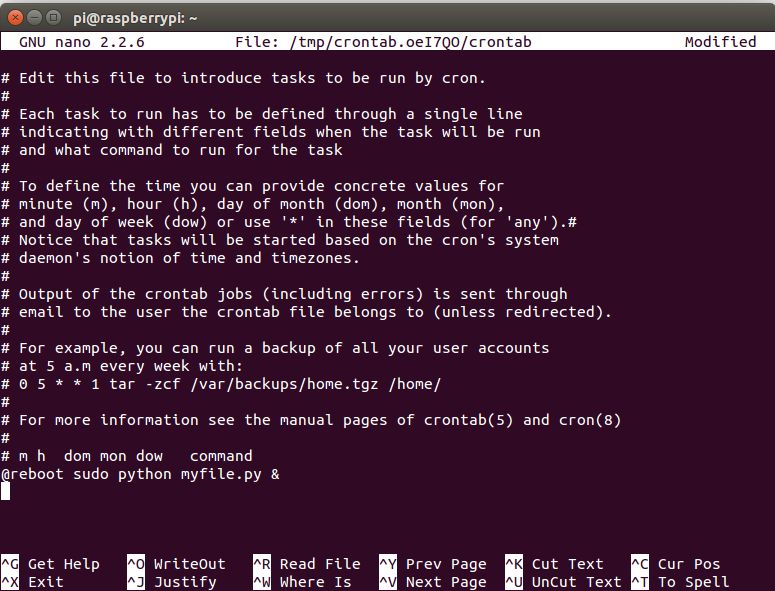
\includegraphics[scale=.5]{run-script-python/images/auto-run-python-1}
\end{center}
\end{figure}
\item Nhấn \verb|Ctrl - X - Y| để lưu lại nội dung thay đổi và thoát.
\item Khởi động lại Pi: \verb|sudo reboot|.
\end{itemize}
Nói thêm về \verb|cron|\footnote{\textsf{https://embeddedday.com/projects/raspberry-pi/a-step-further/running-python-script-at-boot/}} \verb|cron| là một lịch trình, được khai báo với cú pháp sau:
\begin{lstlisting}[language=bash]
1 2 3 4 5 /path/to/command arg1 arg2
\end{lstlisting}
Ý nghĩa của các tham số:
\begin{itemize}
\item \verb|1 = Minutes (0 – 59)|
\item \verb|2 = Hours (0 – 23)|
\item \verb|3 = Days (0 – 31)|
\item \verb|4 = Month (0 – 12)|
\item 5 = Day of the week (0 – 7) (Sunday is the 0 day)|
\end{itemize}
Ta có thể thay thế 1 trong 5 tham số trên bằng các tham số dưới đây:
\begin{itemize}
\item \verb|@reboot|	= Run once, at startup.
\item \verb|@yearly|	= Run once a year
\item \verb|@monthly| = Run once a month
\item \verb|@weekly|	= Run once a week
\item \verb|@daily| = Run once a day
\item \verb|@midnight| = Pretty much the same as \verb|@daily|
\item \verb|@hourly|	= Run once an hour
\end{itemize}
\subsection{Sử dụng profile}
Tham khảo tại:

\begin{footnotesize}
\verb|http://www.raspberrypi-spy.co.uk/2015/02/how-to-autorun-a-python-script-on-raspberry-pi-boot/|
\end{footnotesize}

Thực hiện theo các bước sau:
\begin{itemize}
\item Làm cho Pi có thể tự động đăng nhập được (xem \textit{chủ đề \ref{Sub:auto-login} trang \pageref{Sub:auto-login}}).
\item Mở file profile, dùng lệnh: 
\begin{lstlisting}[language=bash]
$ sudo nano /etc/profile
\end{lstlisting}
\item Kéo xuống dòng cuối dòng, thêm nội dụng sau vào file:
\begin{lstlisting}[language=bash]
sudo python /home/pi/myfile.py &
\end{lstlisting}
Ký hiệu \verb|&| có nghĩa là file \verb|myfile.py| sẽ chạy nền.
\item Nhấn \verb|Ctrl - X - Y| để lưu lại nội dung thay đổi và thoát.
\item Khởi động lại Pi: \verb|sudo reboot|.
\end{itemize}
\subsection{Sử dụng cron kết hợp với tạo file .sh}
Tham khảo tại:

\begin{footnotesize}
\verb|http://www.instructables.com/id/Raspberry-Pi-Launch-Python-script-on-startup/?ALLSTEPS|
\end{footnotesize}

Thực hiện theo các bước sau:
\begin{itemize}
\item Tạo một \verb|.sh| (ví dụ: launcher.sh):
\begin{lstlisting}[language=bash]
$ nano launcher.sh
\end{lstlisting}
\item Nội dung file như sau (thay đổi nội dung của ví dụ cho phù hợp):
\begin{lstlisting}[language=bash]
#!/bin/sh
# launcher.sh
# navigate to home directory, then to this directory, then execute python script, then back home

cd /
cd home/pi/bbt  #thu muc chua file .py
sudo python bbt.py #Lenh chay file python
cd /
\end{lstlisting}
Nhấn \verb|Ctrl - X - Y| để lưu và thoát.
\item Làm cho file \verb|.sh| trở thành file thực thi (executable): 
\begin{lstlisting}[language=bash]
$ chmod 755 launcher.sh
\end{lstlisting}
\item Kiểm tra file \verb|.sh| ta vừa tạo có thực thi được không:
\begin{lstlisting}[language=bash]
$ sh launcher.sh
\end{lstlisting}
\item Tạo thư mục \verb|logs| trong thư mục \verb|\home\pi|:
\begin{lstlisting}[language=bash]
$ cd ~
$ mkdir logs
\end{lstlisting}
\item Mở \verb|crom|:
\begin{lstlisting}[language=bash]
$ sudo crontab -e
\end{lstlisting}
\item Thêm file \verb|.sh| vào \verb|cron|:
\begin{lstlisting}[language=bash]
@reboot sh /home/pi/bbt/launcher.sh >/home/pi/logs/cronlog 2>&1
\end{lstlisting}
Nhấn \verb|Ctrl - X - Y| để lưu và thoát.
\item Khởi động lại Pi: \verb|sudo reboot|
\end{itemize}